\documentclass[a4paper,12pt]{article}
\usepackage{amsmath}
\usepackage{fullpage}
\usepackage{color}
\usepackage{enumerate}
\usepackage{graphicx}

\begin{document}
\title{Five or More Group Analysis\\ Part Two}
\date{November 30, 2010}
\author{Matt Forbes \\ Nick Fitzgerald \\ KC Faulkner \\ Chris Erickson}
\maketitle

\section*{Definitions}
\begin{tabular}{r l}
    Queue:& List of marbles dropping on the board in the next turn. \\
    Group:& A set of same-color marbles on the board that are in an\\
    {}& unobstructed row of 5, but not necessarily touching. \\
    Attach:& Moving a marble to a group's edge.\\
    Completed:& When a group gets five marbles in a row and is taken off the board.\\
    k-Connected:& There are k acyclical paths between a marble and an associated group.\\
    Blocked:& There are no paths between this marble and an associated group.\\
    Region:& Continous unoccupied area on the board. 
    
\end{tabular}


\section*{Goals}

To be clear, we are optimizing for average longevity and points per
game. This contrasts with the approach of taking high risks and
attempting to get an incredible amount of points while failing
frequently; betting on the high risk and high reward route. We are
taking the safe route, so to speak.

We recognize that you do get more points for removing lines of length
greater than the minimum 5, however you shouldn’t prioritize this
technique. The problem is that it sets you up to lose access to that
group when a new marble is spawned in a place that you had reserved
for one of your final marbles. Now, not only can you not get the 6 or
more marbles you were stacking up, but it is possible you cannot even
get the original 5. This is too much of a risk, and will not pay out
in the long term.


\section*{Group Selection}

Ranked in order of highest priority. When multiple color groups match
a rule, the use the list of tie breaking rules, or continue to the
next rule if no rules break the tie, similar to the way which Bucket
Sort operates.

\begin{enumerate}[1)]

    \item Choose a group that has the possibility of being completed with one available move.

    \item Group with the most marbles in it. Break ties by:
        \begin{enumerate}[a)]
            \item Has the most same-colored connected marbles on the board.
            \item Has the most same-colored marbles in the queue. 
        \end{enumerate}

    \item If no groups have conected marbles, then we should start a new group, rules for which
        color and where to start it are discussed below.

\end{enumerate}

Because we are not going out of our way to to get groups of 6 or more,
the obvious choice is to complete a group as soon as possible. We
should always try and complete one specific group so that we can clear
its marbles and open the board up because that increases the longevity
of our game, and thus the amount of points we can gain.

\section*{Actual Marble Selection}

After deciding which group to move, these are the rules on how to pick which marble should be moved to the group
if there are multiple options. These rules also discuss which side of the group the marble should be attached to.

\begin{enumerate}[1)]
    
    \item Pick the marble that would open up the most paths on the board when moved. 
    \item Prioritize marbles that open up paths to other large groups.
    \item Pick marbles that have small k-connections. They are more
      likely to be blocked by incoming marbles from the queue.

\end{enumerate}

\section*{How to Move a Selected Marble}

\begin{enumerate}[1)]
    \item Attach marbles to a space in a  group that has the least
      paths to it. That position is more likely to become blocked by the
      incoming marbles.
    \item Don't attach a marble to the side of a group if that move
      would divide a region (unless that move will complete the group).
      
\end{enumerate}

Our primary goals of marble selection are to aid in the completion of
the largest groups and to keep the board open and clear. The reason
for attaching marbles to the side that is more blocked off is that
after your turn it will be harder to move marbles to that group, so
you sould take advantage of the crowded areas before they are blocked
off and inaccessible.

\section*{Starting a group}

These are guidelines about when no groups are ideal or available, so we need to start a new one.

\begin{enumerate}[1)]
    
    \item Pick the color that has the most same-color connected
      marbles on the board that has sufficient room to be completed.
    \item Pick a base marble which has the most connected marbles of
      the same color and  has sufficient room to complete the
      group. Then pick the marble with smallest k-connection to move
      to it. This marble is the most likely to be blocked after the
      incoming marbles are dropped.
    \item Avoid starting diagonal groups. The rectangular area
      occupied by a diagonal group is completely unavailable to other
      horizontal and vertical groups. While a vertical or horizontal
      group occupies at most 5 squares, a diagonal group occupies 25.

\end{enumerate}

This also ties in to our technique of completing groups as fast as
possible. We are only picking groups that have a high potential of
being completed in as few turns as possible. We are estimating
potential by whether there are enough marbles on the board or in the
queue, and if they are even currently connected.

\pagebreak

\section*{Special Cases}

\begin{enumerate}[1)]

  \item

    Our heuristic would notice that there's more greens on the board
    than any other color, and therefore pick that as the group to work
    with. The best place to move a green to would be the space labeled
    with a 1. Our choice would be to move the light blue marble to
    position 2. It accomplishes more than simply moving a green. There
    are three light blues in the queue that are very unlikely to be
    blocked from the group when they are dropped. It also frees up the
    already started yellow group which can now build in to the center.
    
    \vspace{1in}
    
    \begin{center}
      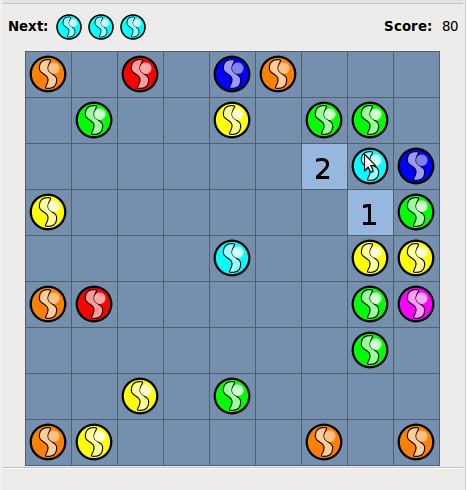
\includegraphics[width=4.5in, height=4.5in, keepaspectratio=true]{image/case1.png}
    \end{center}

\pagebreak
    
  \item

    According to our heuristic, we should move a green marble to the
    position marked with a 1. It has fewer paths to it, and is more
    likely to become blocked from a queue-drop. It would be more
    logical in the long run to move to position 2, which leaves more
    possibilities for the group to be completed.

    If we were to move the marble to position 2, there are less
    combinations of queue drops that could block the reminaing green
    marbles from the group than if we moved to position 1. In the case
    of position 1, the group could be blocked with just one dropped
    marble, while position 2 depends on where two of the three queued
    drop.

    \vspace{1in}
    
    \begin{center}
      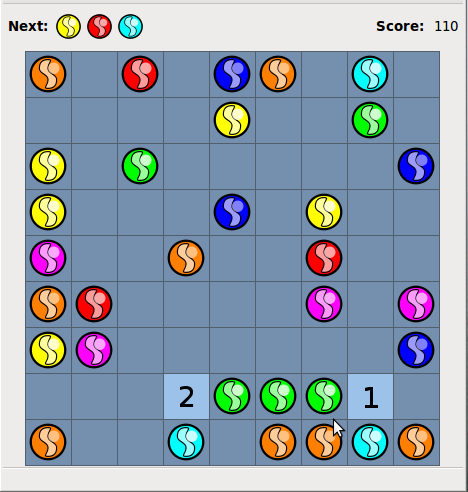
\includegraphics[width=4.5in, height=4.5in, keepaspectratio=true]{image/case2.png}
    \end{center}

\pagebreak

  \item

    The heuristic would not suggest moving the marble to the position
    marked 1, but that is the more logical place to move. It divides a
    region on the right side of the board, but there will be many more
    paths that will complete the red group on the next turn. If we
    were to move to position 2, we couldn't finish the group without
    moving other marbles.

    \vspace{1in}

    \begin{center}
      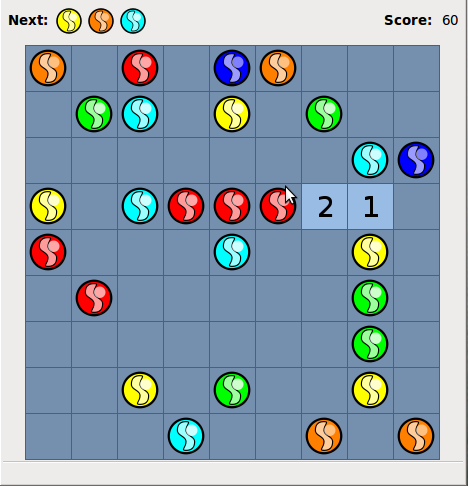
\includegraphics[width=4.5in, height=4.5in, keepaspectratio=true]{image/case3.png}
    \end{center}
  
\end{enumerate}

\end{document}
